% !TEX program = xelatex
% !TEX encoding = UTF-8

%%%%%%%%%%%%%%%%%%%%%%%%%%%%%%%%%%%%%%%%%%%%%%%%%%%%%%%%%%%%%%%%%%%%%%%%%%%%%%%%
%%%%%%%%%%%%%%%%%%%%%%%%%%%%%%%%%%%%%%%%%%%%%%%%%%%%%%%%%%%%%%%%%%%%%%%%%%%%%%%%
%%
%% 
%% File Name:           main.tex Tex文件 文档编译入口文件
%% Author:              itanggx@gmail.com / tgx126sicnu@126.com
%% Created On:          2022-09-14 16:36
%% Last Modified By:    tang-guoxin
%% Description:         一个基于 TexLive 的 SICNU 模板, 使用该模板的要求为 TeXLive 版本大于等于 2021-11-15, 编译方式必须为 xelatex
%%                      第一行为Magic注释, 该注释将会使得计算机自动选用xelatex
%% Project Adress:      www.github.com/tang-guoxin/sicnu-template
%% Other:               .vscode 文件夹下的 setting.json 文件为 vscode 配置文件, 在里面已经定义了编译方式和步骤, 不能删除
%%
%%%%%%%%%%%%%%%%%%%%%%%%%%%%%%%%%%%%%%%%%%%%%%%%%%%%%%%%%%%%%%%%%%%%%%%%%%%%%%%%
%%%%%%%%%%%%%%%%%%%%%%%%%%%%%%%%%%%%%%%%%%%%%%%%%%%%%%%%%%%%%%%%%%%%%%%%%%%%%%%%
\documentclass{sicnu}

\begin{document}
    %% ! 论文基本信息
    % todo 中文标题
    % // \ChineseTitle{一二三四五六七八九一二三四五六七八九一二三四五六七八九ABCDEFG}
    \ChineseTitle{一二三四五六七八九一二三四五六七八九九}
    % todo 英文标题
    \EnglishTitle{Time New Roman Time New Roman Time New Roman Time New Roman}
    % todo 中文作者姓名
    \ChineseAuthorName{魔法学徒}
    % todo 英文作者姓名
    \EnglishAuthorName{Magic Apprentice}
    % todo 学号
    \StudentNumber{20200801000}
    % todo 中文导师姓名
    \ChineseSupervisor{西弗勒斯·斯内普}
    % todo 英文导师姓名
    \EnglishSupervisor{Severus Snape}
    % todo 中文专业
    \ChineseMajorName{黑魔法}
    % todo 英文专业
    \EnglishMajorName{Dark Magic}
    % todo 研究方向
    \ResearchDirection{黑魔法防御术和魔药学}
    % todo 学院
    \CollegeName{斯莱特林}
    % todo 提交日期
    \ThesisSubmissionDate{\today}
    % todo 答辩日期
    \ThesisDefenseDate{2022年9月23日}

    %% ! 生成封面, 独创性声明和授权书
    \MakeTitlePage
    %% ! 摘要
    \begin{ChineseAbstract}
    自$2014$年起,CTex已不再维护和更新,然而现在流传下来的TeX模板仍然是基于CTex的模板。最新的一个版本是$2014$年的版本,最古老的可以追溯到$2004$年。TeXLive是未来的趋势。
    
    在过去的CTex模板中,仅仅是将模板元素的定义放到一个\verb|.tex|文件中。并且没有封装所有的定义和设置,在主程序中仍然有第三方包的导入和全局全局定义。这个模板将使用最简洁的代码来帮助作者完成你的毕业论文。只需要一行代码:\verb|\documentclass{sicnu}|。恭喜你,你已经完成了整个文档的所有设定,因为所有的元素都已被封装进了\verb|sicnu.cls|类中。

    这个模板封装了约$40$个包,新定义了$29$个可供直接调用的外部指令,新定义了$5$个的环境,重定义了$7$个环境。将来可能会对模板进行增删调补。并且分离了章节,而不是一股脑的放到一个文件中。这可以提高我们写作的专注力,同时便于检查错误和修改文章。或许听着有点多,但事实上这些命令和环境仅仅是帮助作者写入论文题目以及摘要关键词等信息,甚至你完全不需要阅读使用说明也能看懂这个指令做了什么。\textcolor{red}{你还可以通过预留的指令轻松将模板改成博士论文模板而不需要修改源代码。}

    最后,参考文献的引用和生成是区别于CTex模板的最大改进。现在文献将会根据引用的顺序在末尾自动排序(以前的模板需要手动排序)。并且使用了(GB/T 7714--2005)规范。

    \ChineseKeyword{关键词1;关键词2;关键词3;关键词4;关键词5}
\end{ChineseAbstract}

\begin{EnglishAbstract}
    Since $2014$, CTex is no longer maintained and updated, however, the TeX templates that have been handed down are still based on CTex. The latest version is the $2014$version, and the oldest version dates back to the $2004$year. TeXLive is the future.

    In the past CTex templates, merely defines the template elements into a \verb|.tex| file. And instead of encapsulating all the definitions and Settings, there are still third-party package imports and global global definitions in the main program. This template will use the most concise code to help the author complete your thesis. All it takes is one line of code: \verb|\documentclass{sicnu}|. Congratulations, you have completed the entire document set, because all of the elements have been encapsulated into the \verb|sicnu.cls| classes.

    This template encapsulates about $40$ packages, defines $29$ external instructions that can be called directly, defines $5$environments, and redefines $7$ environments. The template may be added or deleted in the future. And separate chapters instead of putting them all in one file. This improves our ability to focus on writing, and makes it easier to check for errors and revise. This may sound like a lot, but the fact is that these commands and environments just help the author write the title and abstract keywords, and you don't even need to read the instructions at all to understand what the command does. \textcolor{red}{You can also easily change the template into a doctoral thesis template with reserved instructions without changing the source code. }

    Finally, reference citations and generation are the biggest improvements that distinguish them from CTex templates. References will now be automatically sorted at the end by the order they are cited (previous templates required manual sorting). The specification (GB/T 7714--2005) is also used.

    \EnglishKeyword{Keyword1;Keyword2;Keyword3;Keyword4;Keyword5}
\end{EnglishAbstract}


    %% ! 生成目录
    \GenerateContents
    \cleardoublepage
    %% ! 生成算法, 图片以及表格清单
    \GenerateFTAList

    %% ! 第一章
    \section{开始使用}\label{sec:intro}

\par 这一章的主要目的是为了介绍什么是\LaTeX,\verb|sicnu.cls|文档类的基本使用方法以及整个项目的布局。顺便生成一些表格和图片便于测试整个文档以及用户快速对模板的修改和使用。

\subsection{什么是\LaTeX }\label{sec:intro:p1}
\par TEX是高德纳(Donald E. Knuth)为排版文字和数学公式而开发的软件\cite{texbook}。\LaTeX 是一种使用TEX程序作为排版引擎的格式,可以粗略地将它理解成是对TEX的一层封装。我们当前使用的版本是\LaTeXe,事实上{\LaTeX}3已经发布很多年了,但是\LaTeXe 仍然是目前使用最广泛的版本。点击\href{https://www.latex-project.org/latex3/}{传送门}查看关于{\LaTeX}3的更多信息。

\par 下面介绍常见的\LaTeX 引擎, \LaTeX 发行版以及 \LaTeX 编辑器的区别与联系。请看图\ref{fig:texbase}:
\begin{figure}[H]
    \centering
    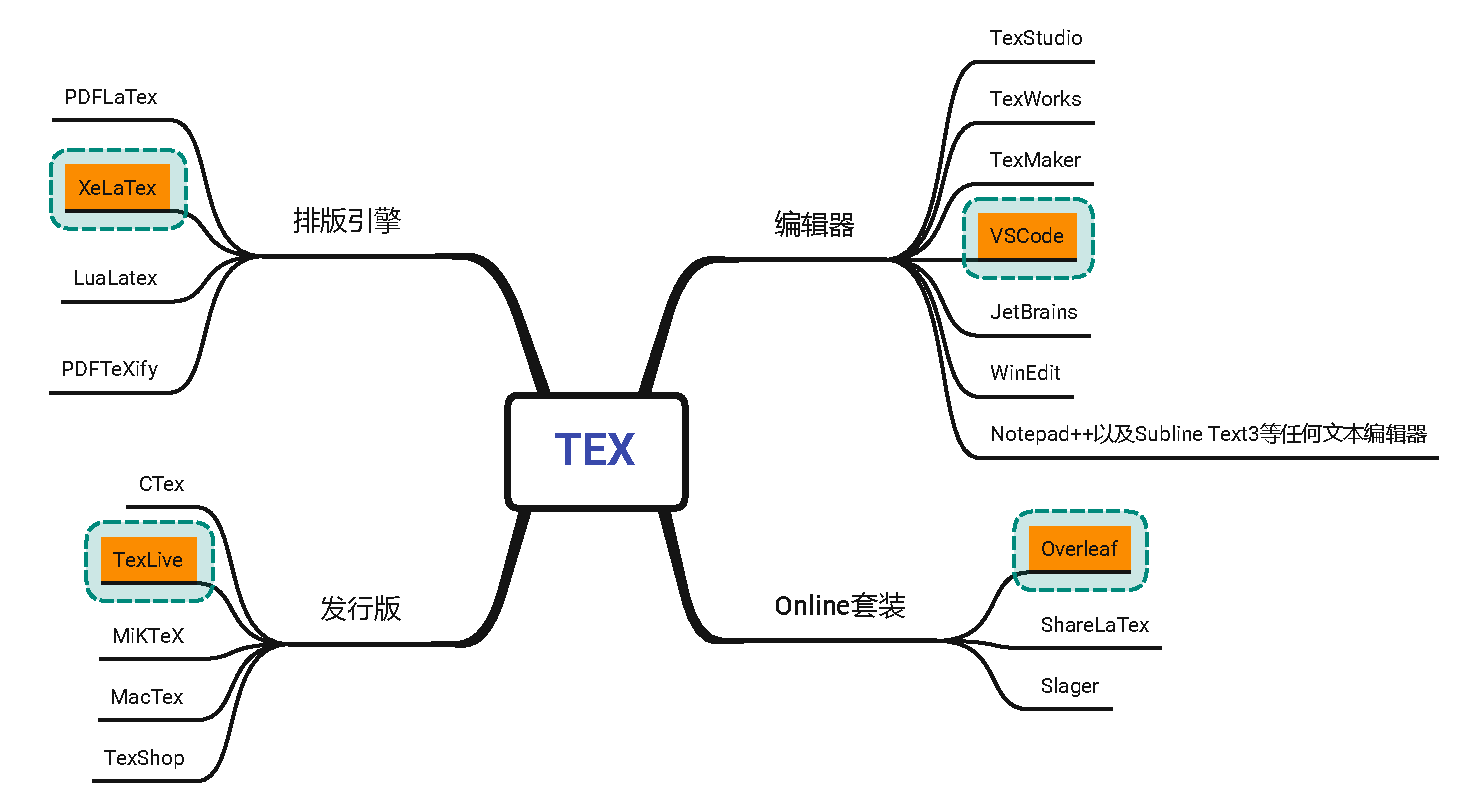
\includegraphics[scale=0.5]{./img/TEX.pdf}
    \caption{TeX的基础知识}
    \label{fig:texbase}
\end{figure}

\par \textcolor{red}{这个项目使用的\LaTeX 发行版为TeXLive2021,编译引擎为XeLaTex,开发环境为VSCode。}需要注意的是,尽管TeXLive支持macOS和Linux,但TeX并不是一个跨平台语言,\textcolor{red}{所以Mac和Linux用户将无法轻松的使用这个模板。}如果你要使用这个模板,下面的条件需要尽可能的满足:

\begin{tcolorbox}[colback=gray!10,
    colframe=black,
    width=16cm,
    arc=1mm, auto outer arc,
    boxrule=0.5pt,]
    \begin{itemize}
        \item 操作系统为Windows7以上。
        \item $\mathrm{TexLive~~Version >= 2021}$,更高或更低的版本也应该能完成编译,这只是成功的充分条件,但是禁用CTex。
        \item 编辑器推荐等级:$\mathrm{VSCode > TexStudio > TexWorks > TexMaker}$,其中TeXLive自带TexWorks编辑器。禁用WinEdit。
        \item 编译方式为XeLaTex。
        \item 如果你不想安装TeXLive,请使用\textcolor{red}{Overleaf或ShareLaTex},通过它们你可以直接从\href{github}{github}上导入这个项目在线编译。
    \end{itemize}
\end{tcolorbox}
如果你点电脑上没有安装TeXLive,请查看\href{https://www.bilibili.com/video/BV1tg4y1B7f3/?spm_id_from=333.337.search-card.all.click&vd_source=758c464d5854d0b3d36de4033fcbdc7a}{\LaTeX 工作室}制作的安装教程:\url{https://www.bilibili.com/video/BV1tg4y1B7f3/?spm_id_from=333.337.search-card.all.click&vd_source=758c464d5854d0b3d36de4033fcbdc7a}。这个教程前半部分介绍TeXLive的安装,后半部分介绍了命令行的用法,只需要完成前半部分教程即可。

\subsection{sicnu.cls的基本用法}

\par \verb|sicnu.cls|文件目前包括新定义了$29$个可供直接调用的外部指令,新定义了$5$个的环境,重定义了$7$个环境。内部命令和宏不在此处列出,如果有这些定义解决不了的问题请查看源码。图\ref{fig:basevar}是主程序入口,它的结构不会因为你的论文内容而改变。
\begin{figure}[H]
    \centering
    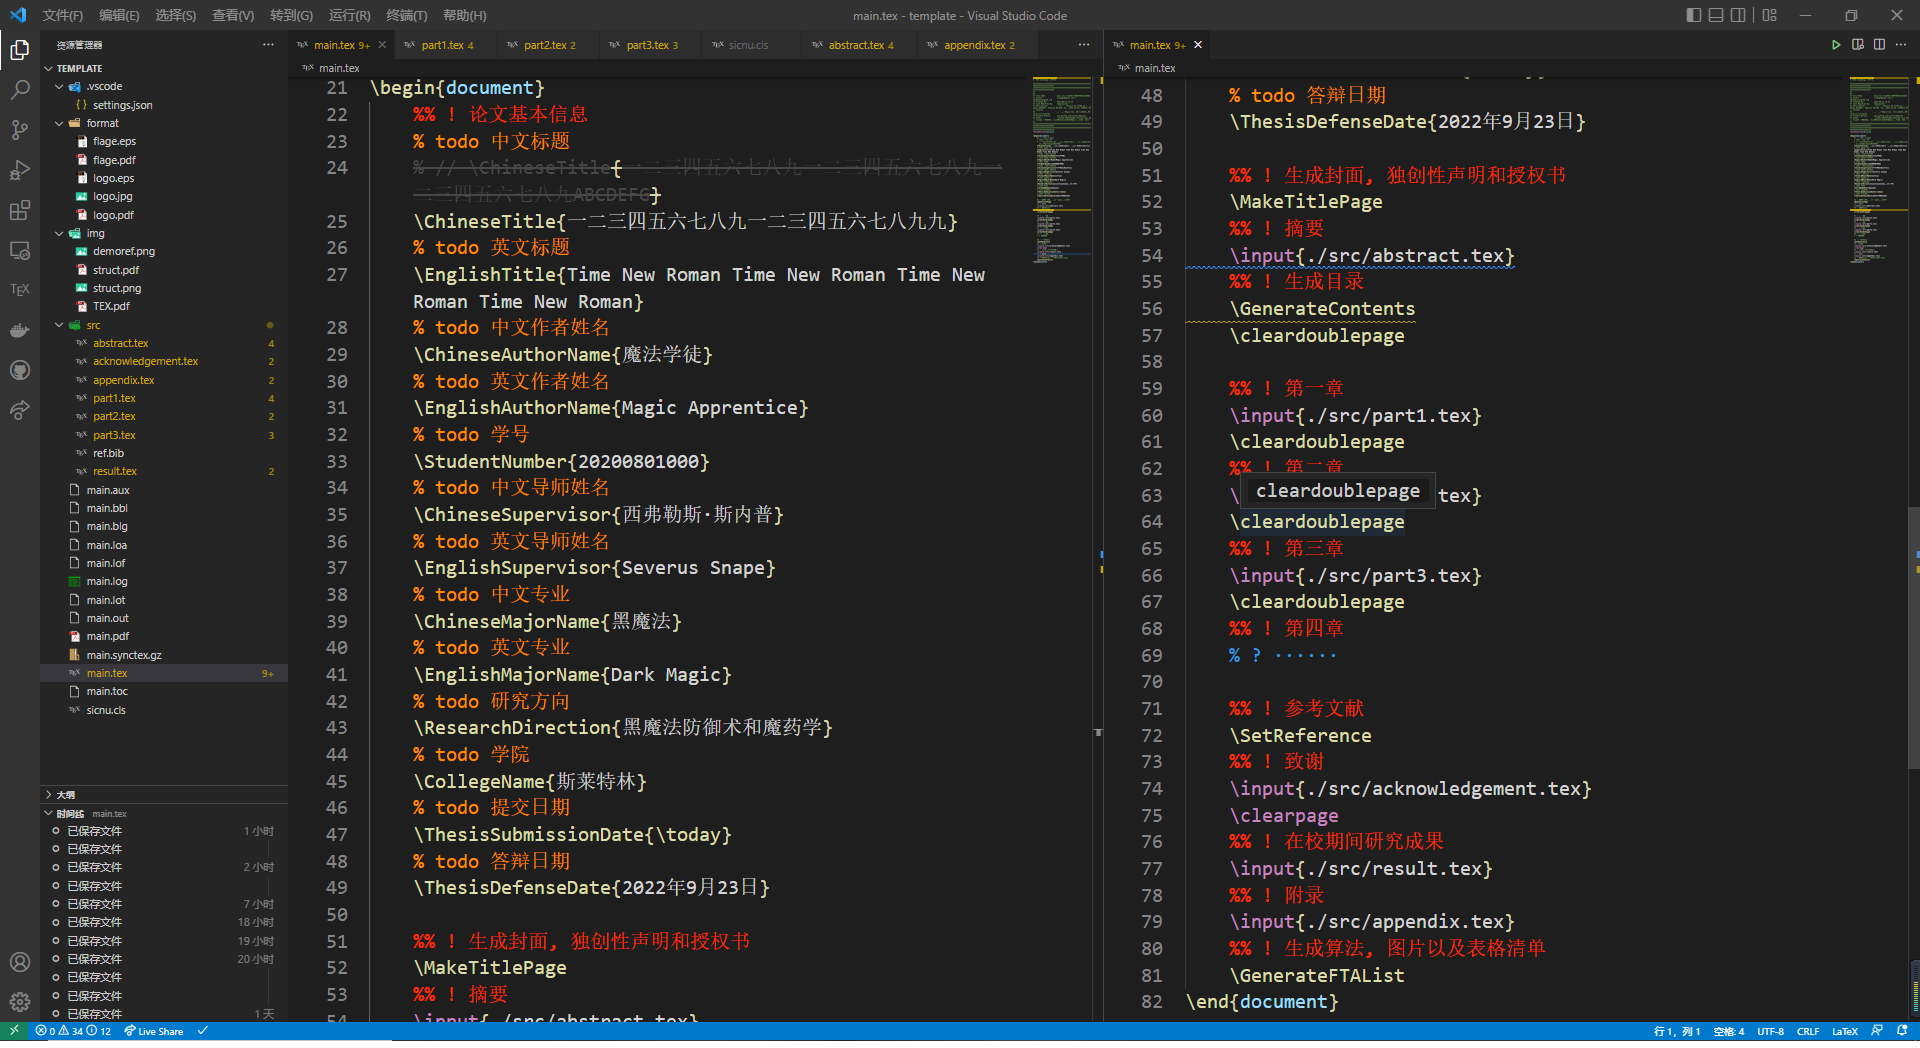
\includegraphics[scale=0.3]{img/struct.png}
    \caption{文档的基本元素设置}
    \label{fig:basevar}
\end{figure}
以上这些命令都是最基本的命令,你无需记住它,而它们也只会使用一次。看懂了这张图,那么这个模板你已会$80\%$了。诸如分类号和学校代码等也提供了指令修改它,但是默认值就是SICNU,故无特殊需要可以不用在意它。第二章会列出所有可供调用的指令和环境,以供后期调试和使用。

\subsection{项目布局}
\par 也许你已经发现了,图\ref{fig:basevar}中并没有任何正文的内容。它们都是通过如第$58$行的\verb|\input{path}|导入相应的文件。文章的每一章都将使用一个独立的文件保存,而不是一股脑的把所有内容塞到一个文件中,这将方便我们检查错误和提高专注力。结合图\ref{fig:basevar}和图\ref{fig:projstru}以及你的论文,你就知道你需要修改模板的哪个地方了。

\begin{figure}[H]
    \centering
    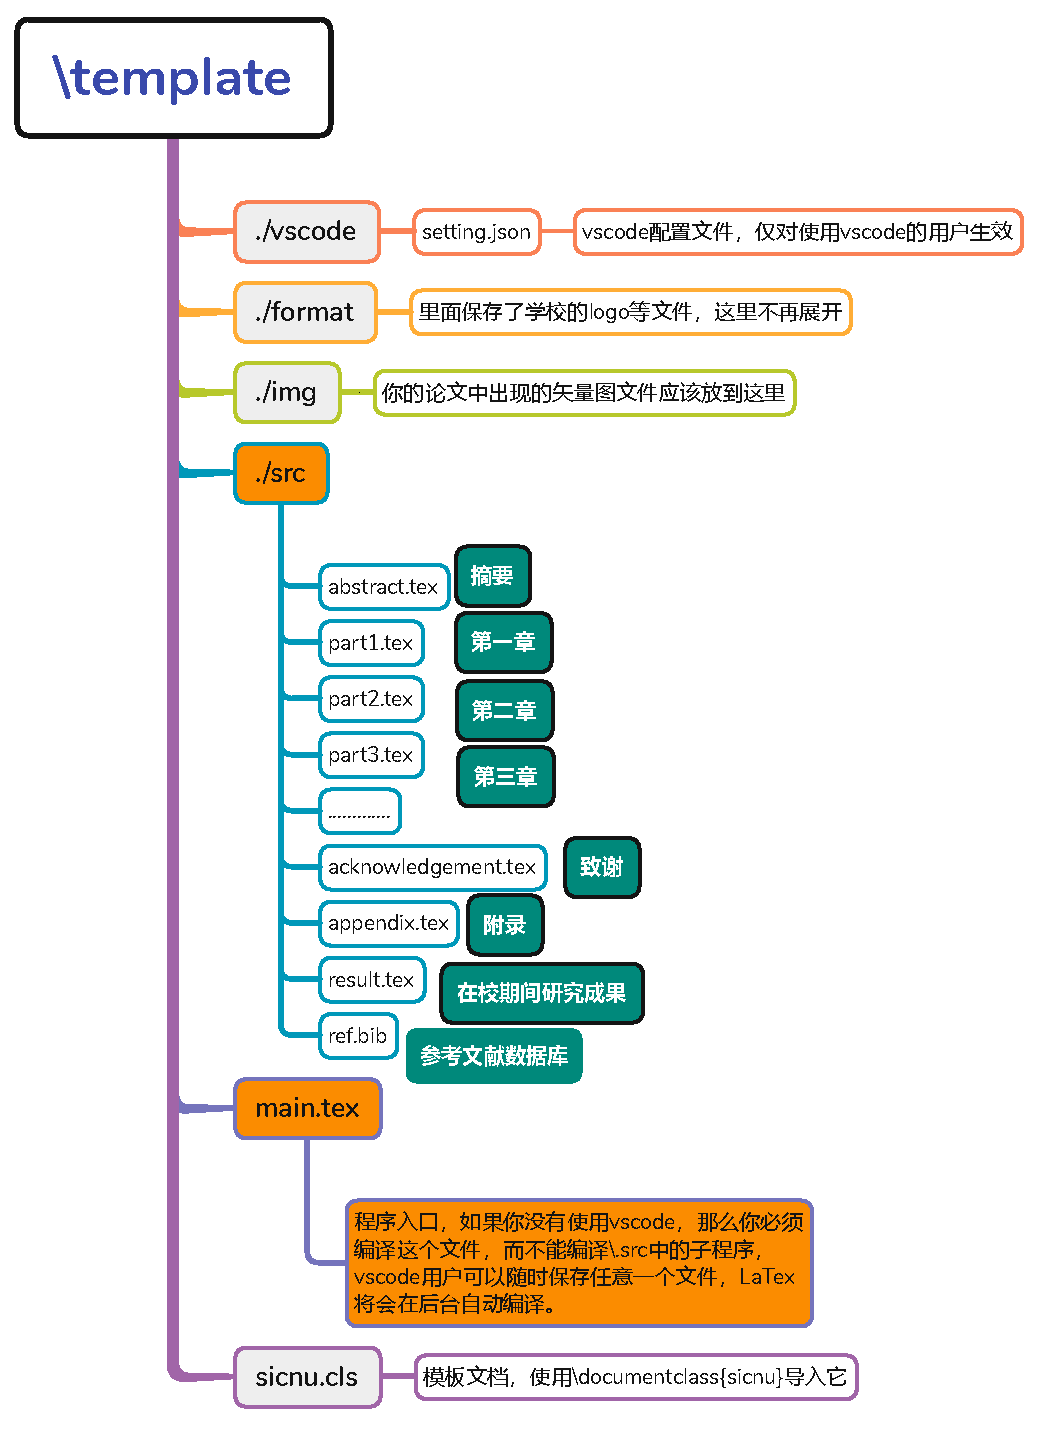
\includegraphics[scale=0.8]{img/struct.pdf}
    \caption{项目布局}
    \label{fig:projstru}
\end{figure}

\subsection{轻松引用参考文献}
看到这里,你已经学会了这个模板$90\%$的内容了。接下来,学习如何使用数据库来管理你的参考文献。\textcolor{red}{使用数据库管理和引用参考文献的方式可以避免手动输入文献和文献引用排序的问题,这是以前的CTex模板最让人难以忍受的地方。}将你的参考文献放到\verb|ref.bib|文件中,形如:
\begin{tcolorbox}[colback=gray!10,
    colframe=black,
    width=16cm,
    arc=1mm, auto outer arc,
    boxrule=0.5pt,]
    \begin{verbatim}
        % ./src/ref.bib
        @article{tpe,  % 引用的别名
            title={Algorithms for hyper-parameter optimization},
            author={Bergstra, James and Bardenet,
                R{\'e}mi and Bengio, Yoshua and K{\'e}gl, Bal{\'a}zs},
            journal={Advances in neural information processing systems},
            volume={24},
            year={2011}
        }
        @article{lecun, % 引用的别名
            title={Deep learning},
            author={LeCun, Yann and Bengio, Yoshua and Hinton, Geoffrey},
            journal={nature},
            volume={521},
            number={7553},
            pages={436--444},
            year={2015},
            publisher={Nature Publishing Group}
        }
    \end{verbatim}
\end{tcolorbox}
这些信息非常容易获取,知网,百度学术,Google Scholar都有复制粘贴的选项,如图\ref{fig:citebib}所示。
\begin{figure}[H]
    \centering
    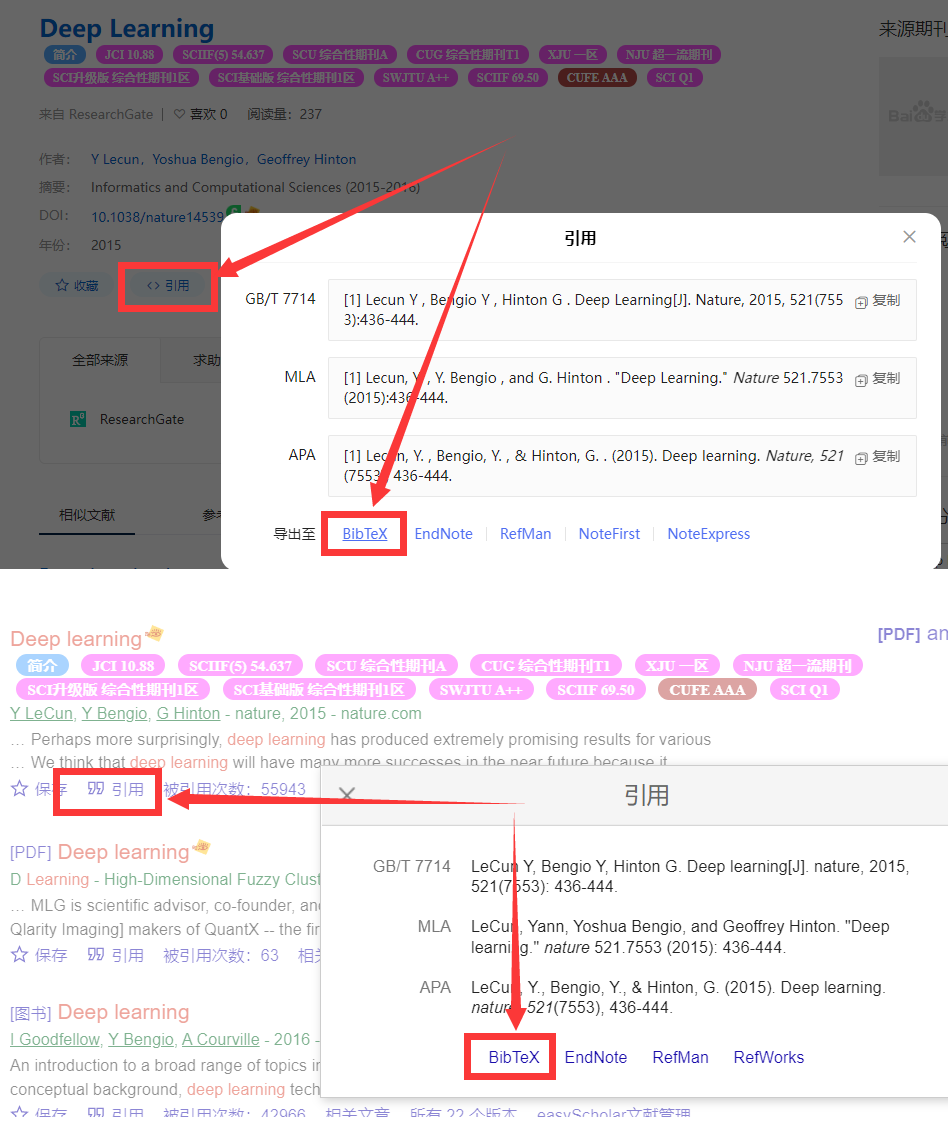
\includegraphics[scale=0.3]{img/demoref.png}
    \caption{如何复制参考文献的引用格式}
    \label{fig:citebib}
\end{figure}

将bib格式的文献复制粘贴到\verb|ref.bib|文件中后,接下来使用\verb|\cite{tpe, lecun}| \cite{tpe, lecun}引用这两个文献。使用这种方式引用文献有以下好处,这是之前CTex模板没有解决的问题:
\begin{tcolorbox}[colback=gray!10,
    colframe=black,
    width=16cm,
    arc=1mm, auto outer arc,
    boxrule=0.5pt,]
    \begin{itemize}
        \item 文献会根据你在正文中引用的顺序自动在末尾产生参考文献页。(以前的模板需要手动排序,比如你在第$7$个文献后又引用了一个新的文献,那么后面的文献你都要手动把序号$+1$。现在,你只管引用,文献排序将自动完成。)
        \item 文献引用规范为(GB/T 7714--2005),以前的模板有的没有遵循这个规则。
        \item 使用数据库管理文献避免了你去手动排版文献格式,复制粘贴更不容易出错。
    \end{itemize}
\end{tcolorbox}


    \cleardoublepage
    %% ! 第二章
    \section{sicnu.cls的指令和环境}\label{sec:cml}
\subsection{基本指令}
\begin{tcolorbox}[colback=gray!10,
    colframe=black,
    width=16cm,
    arc=1mm, auto outer arc,
    boxrule=0.5pt,]
    
    \begin{enumerate}
        \item \verb|\ChineseTitle{key}| 设置中文论文名称。
        \item \verb|\EnglishTitle{key}| 设置英文论文名称。
        \item \verb|\ChineseAuthorName{key}| 设置中文作者姓名。
        \item \verb|\EnglishAuthorName{key}| 设置英文作者姓名。
        \item \verb|\Classification{key}| 设置分类号,默认为O21。
        \item \verb|\SecretLevel{key}| 设置密级,默认为公开。
        \item \verb|\UnitCode{key}| 设置单位代码,默认为10636。
        \item \verb|\StudentNumber{key}| 设置单位代码,默认为学号。
        \item \verb|\ChineseSupervisor{key}| 设置中文导师姓名。
        \item \verb|\ChineseSupervisor{key}| 设置英文导师姓名。
        \item \verb|\ChineseMajorName{key}| 设置中文专业名。
        \item \verb|\EnglishMajorName{key}| 设置英文专业名。
        \item \verb|\ResearchDirection{key}| 设置研究方向。
        \item \verb|\CollegeName{key}| 设置所在学院。
        \item \verb|\ThesisSubmissionDate{key}| 设置论文提交日期。
        \item \verb|\ThesisDefenseDate{key}| 设置论文答辩日期。
        \item \verb|\GenerateContents| 在指定位置生成目录。
        \item \verb|\EnglishKeyword{key}| 设置英文关键词,不同关键词用逗号分开。
        \item \verb|\ChineseKeyword{key}| 设置中文关键词,不同关键词用逗号分开。
        \item \verb|\SetReference| 在指定位置生成参考文献。
        \item \verb|\MakeTitlePage[#1]| 在指定位置生成生成封面, 独创性声明和授权书。带有一个可选参数,设置为$1$改为博士学位论文,默认为$0$。
        \item \verb|\GenerateFTAList| 生成图表和算法清单
    \end{enumerate}

\end{tcolorbox}

\subsection{扩展指令}
\begin{tcolorbox}[colback=gray!10,
    colframe=black,
    width=16cm,
    arc=1mm, auto outer arc,
    boxrule=0.5pt,]
    
    \begin{enumerate}
        \item \verb|\NewEmptypPge| 增加一页空白页,并且不带页眉和页脚。\verb|\cleardoublepage|将清除偶数页,使得每一章都从奇数页开始。但是会受到pagecounter的影响。而此命令是强制性命令,不区分奇偶。
        \item \verb|\EqualityNum{#1}{#2}| 比较两个数的大小,需要配合定义的宏\verb|\if@twonumcmp|一起使用。(这个函数最开始是实现标题自动换行的部分逻辑,后面已经使用更加有效的方式处理。)
        \item \verb|\DegreeLevel{#1}| 设置偶数页页眉,博士论文需要使用这个指令,默认为硕士学位论文。
        \item \verb|\SetLinkColor[#1]| 超链接开关,默认打开,设置为$0$关闭。
        \item \verb|\Length{text}| 获取文本长度。(这个函数最开始是实现标题自动换行的部分逻辑,后面已经使用更加有效的方式处理。)
        \item \verb|\newyouyuan{text}| 设置文本为幼圆。
        \item \verb|\newfangsong{text}| 设置文本为仿宋。
        
    \end{enumerate}


\end{tcolorbox}


\subsection{新定义的环境}
\begin{tcolorbox}[colback=gray!10,
    colframe=black,
    width=16cm,
    arc=1mm, auto outer arc,
    boxrule=0.5pt,]

    \begin{enumerate}
        \item 中文摘要环境
\begin{verbatim}
    \begin{ChineseAbstract}
        text......
        \ChineseKeyword{Keyword1;Keyword2;Keyword3;Keyword4;Keyword5}
    \end{ChineseAbstract}
\end{verbatim}
        \item 英文摘要环境
\begin{verbatim}
    \begin{EnglishAbstract}
        text......
        \EnglishKeyword{Keyword1;Keyword2;Keyword3;Keyword4;Keyword5}
    \end{EnglishAbstract}
\end{verbatim}
        \item 致谢环境
\begin{verbatim}
    \begin{MyHeart}
        text......
    \end{MyHeart}
\end{verbatim}
        \item 在校期间研究成果环境,需要配合\verb|\bibentry{key}|一起使用,就和引用参考文献的使用方法一致:\verb|\cite{key}|。
\begin{verbatim}
    \begin{Achievement}
        \item \bibentry{tpe}
        \item \bibentry{lecun}
    \end{Achievement}
\end{verbatim}
        \item 附录环境
\begin{verbatim}
    \begin{Appendix}
        text......
    \end{Appendix}
\end{verbatim}
    \end{enumerate}
\end{tcolorbox}

\subsection{重定义的环境}

\begin{tcolorbox}[colback=gray!10,
    colframe=black,
    width=16cm,
    arc=1mm, auto outer arc,
    boxrule=0.5pt,]

    \begin{enumerate}[itemsep= 10pt, partopsep=10pt]
        \item 定理环境
\begin{verbatim}
    \begin{theorem}[theorem name]
        定理内容, 可以嵌套公式和证明环境.
    \end{theorem}
\end{verbatim}
        \item 推论环境
\begin{verbatim}
    \begin{corollary}[corollary name]
        推论内容, 可以嵌套公式和证明环境.
    \end{corollary}
\end{verbatim}
        \item 例子环境
\begin{verbatim}
    \begin{example}[example name]
        例子内容, 可以嵌套公式和证明环境.
    \end{example}
\end{verbatim}
        \item 引理环境
\begin{verbatim}
    \begin{lemma}[lemma name]
        引理内容, 可以嵌套公式和证明环境.
    \end{lemma}
\end{verbatim}
        \item 命题环境
\begin{verbatim}
    \begin{proposition}[proposition name]
        命题内容, 可以嵌套公式和证明环境.
    \end{proposition}
\end{verbatim}
        \item 定义环境
\begin{verbatim}
    \begin{definition}[definition name]
        定义内容, 可以嵌套公式和证明环境.
    \end{definition}
\end{verbatim}
        \item 证明环境
\begin{verbatim}
    \begin{proof}证明内容......\end{proof}
\end{verbatim}
    \end{enumerate}
\end{tcolorbox}

    \cleardoublepage
    %% ! 第三章
    \section{简单的案例}

\subsection{数学环境测试}

\begin{definition}[菲波那切数列]
    令$F_0=0,F_1=1$,称由如下递推定义的数列
    \begin{equation}
        F_k = F_{k-1} + F_{k-2}.
    \end{equation}
    为斐波那契数列。
\end{definition}

\begin{theorem}[斐波那契的通项公式]
    斐波那契数列通项公式是一个典型的由无理数表示有理数的公式:
    \begin{equation}
        F_k=\frac{1}{\sqrt{5}}\left( \left( \frac{1+\sqrt{5}}{2} \right) ^k-\left( \frac{1-\sqrt{5}}{2} \right) ^k \right) 
    \end{equation}
    \begin{proof}
        \begin{equation}
            \begin{aligned}
                F_k&=\frac{1}{\sqrt{5}}\left( \left( \frac{1+\sqrt{5}}{2} \right) ^k-\left( \frac{1-\sqrt{5}}{2} \right) ^k \right)\\
                &=\frac{1}{\sqrt{5}}\left( \left( \frac{1+\sqrt{5}}{2} \right) ^{k-2}\left( \frac{1+\sqrt{5}}{2} \right) ^2-\left( \frac{1-\sqrt{5}}{2} \right) ^{k-2}\left( \frac{1-\sqrt{5}}{2} \right) ^2 \right)\\
                &=\frac{1}{\sqrt{5}}\left( \left( \frac{1+\sqrt{5}}{2} \right) ^{k-2}\left( \frac{3+\sqrt{5}}{2} \right) -\left( \frac{1-\sqrt{5}}{2} \right) ^{k-2}\left( \frac{3-\sqrt{5}}{2} \right) \right)\\
                &=\frac{1}{\sqrt{5}}\left( \left( \frac{1+\sqrt{5}}{2} \right) ^{k-2}\left( \frac{1+\sqrt{5}}{2}+1 \right) -\left( \frac{1-\sqrt{5}}{2} \right) ^{k-2}\left( \frac{1-\sqrt{5}}{2}+1 \right) \right)\\
                &=\frac{1}{\sqrt{5}}\left( \left( \frac{1+\sqrt{5}}{2} \right) ^{k-1}+\left( \frac{1+\sqrt{5}}{2} \right) ^{k-2}-\left( \frac{1-\sqrt{5}}{2} \right) ^{k-1}-\left( \frac{1-\sqrt{5}}{2} \right) ^{k-2} \right)\\
                &=\frac{1}{\sqrt{5}}\left( \left( \frac{1+\sqrt{5}}{2} \right) ^{k-1}-\left( \frac{1-\sqrt{5}}{2} \right) ^{k-1}+\left( \frac{1+\sqrt{5}}{2} \right) ^{k-2}-\left( \frac{1-\sqrt{5}}{2} \right) ^{k-2} \right)\\
                &=\frac{1}{\sqrt{5}}\left( \left( \frac{1+\sqrt{5}}{2} \right) ^{k-1}-\left( \frac{1-\sqrt{5}}{2} \right) ^{k-1} \right) +\frac{1}{\sqrt{5}}\left( \left( \frac{1+\sqrt{5}}{2} \right) ^{k-2}-\left( \frac{1-\sqrt{5}}{2} \right) ^{k-2} \right)\\
                &=F_{k-1}+F_{k-2}\\
            \end{aligned}
        \end{equation}
    \end{proof}
\end{theorem}

\begin{corollary}[关于斐波那契数列的一些等式]
    \begin{equation}
        F_{k+1}F_{k-1}-F_{k}^{2}=(-1)^k
    \end{equation}
    \begin{equation}
        F_{n+m}=F_mF_{n+1}+F_{m-1}F_n
    \end{equation}
    \begin{equation}
        \lim_{k\rightarrow \infty} \frac{F_k}{F_{k+1}}=\lim_{k\rightarrow \infty} \frac{F_{k+1}}{F_{k+2}}=\frac{\sqrt{5}-1}{2}
    \end{equation}
    \begin{equation}
        \sum_{i=1}^n{F_i}=F_{n+2}-1
    \end{equation}
    \begin{equation}
        \sum_{i=1}^n{F_{2n-1}}=F_{2n}
    \end{equation}
    \begin{equation}
        \sum_{i=1}^n{F_{2n}}=F_{2n+1}-1
    \end{equation}
    
\end{corollary}

\begin{lemma}[整数快速幂]\label{lem:lem1}
    设一个正整数$x$的二进制表示为$x=\sum_{i=0}^{n-1}{b_i\times 2^i}$。其中$b_i\in\{0, 1\}$是$x$的第$i$位的二进制值。设另有一正整数$y$,那么$y$的$x$次幂可以表示为:
    \begin{equation}
        y^x=\prod_{i=0}^{n-1}{y^{b_i\times 2^i}}
    \end{equation}
    通过这种计算方式将时间复杂度从$O(n)$降低到$O(\log(n))$。代码实现见附录。
\end{lemma}

\begin{proposition}[矩阵快速幂]
    设$F_n$为斐波那契数列的第$n$项,则有:
    \begin{equation}
        \left[ \begin{array}{c}
            F_n\\
            F_{n-1}\\
        \end{array} \right] =\left[ \begin{matrix}
            1&		1\\
            1&		0\\
        \end{matrix} \right] \times \left[ \begin{array}{c}
            F_{n-1}\\
            F_{n-2}\\
        \end{array} \right] 
    \end{equation}
    更进一步有:
    \begin{equation}
        \left[ \begin{array}{c}
            F_n\\
            F_{n-1}\\
        \end{array} \right] =\left[ \begin{matrix}
            1&		1\\
            1&		0\\
        \end{matrix} \right] ^{n-1}\times \left[ \begin{array}{c}
            F_2\\
            F_1\\
        \end{array} \right] 
    \end{equation}
    令矩阵$\varLambda =\left[ \begin{matrix}
        1&		1\\
        1&		0\\
    \end{matrix} \right] $,则$\varLambda ^n$可以通过与引理\ref{lem:lem1}类似的方法快速计算出。矩阵快速幂求斐波那契数列的第$n$项是目前最快的方法。
\end{proposition}



\begin{example}[P1962~斐波那契数列(洛谷)]
    大家都知道,斐波那契数列是满足如下性质的一个数列:
    \begin{equation}
        F_n=\left\{\begin{array}{r}
            1(n \leq 2) \\
            F_{n-1}+F_{n-2}(n \geq 3)
            \end{array}\right.
    \end{equation}
    请你求出$F_n~\mathrm{mode}~10^9 + 7$的值。时间限制$\mathrm{1.00s}$,内存限制$\mathrm{125.00MB}$。
    \par 对于 $60\%$ 的数据,$1\le n \le 92$;对于 $100\%$ 的数据,$1\le n < 2^{63}$。
    \par \textbf{解:}略......
\end{example}

% \lstinputlisting[breaklines]{source.c}

\subsection{总结与展望}
最后附上常用常用的其它命令,它们都不是这个模板定义的指令或环境。但是lshort-zh-cn文档值的所有人去阅读它,这是一个 \LaTeX 中文教程,内容在100页左右,只需要几个小时你就能理解大部分内容。看懂了之后一般的 \LaTeX 排版不在话下。

\subsubsection{TeXLive包管理器与帮助文档}
\begin{tcolorbox}[colback=gray!10,
    colframe=black,
    width=16cm,
    arc=1mm, auto outer arc,
    boxrule=0.5pt,]
\begin{verbatim}
    tlmgr --version             % 查看TeXLive包管理器的版本
    tlmgr option repository ctan% 更新包
    tlmgr update --self --all   % 更新tmlgr
    texdoc ctex                 % 查看 ctex 宏集帮助文档, 
                                % 这个模板也参考了这个文档
    texdoc xecjk                % 里面有许多中文的额外支持, 如下划线自动换行
    texdoc lshort-zh-cn         % 查看一份不太简短的LaTex2e教程, 100页左右
                                % 看懂这个文档你就可以理解sicnu.cls的80%的内容
                                % 非常适合新手的入门教程
    texdoc [texdoc]             % 随机打开文档或查看所有可选文档
    texdoc package-name         % 查看任一宏包的帮助文档
    xelatex -v                  % 查看xelatex的版本
    latexmk -xelatex main.tex   % 自动编译main.tex文档
\end{verbatim}

\end{tcolorbox}

\subsubsection{已导入的宏包}

% Please add the following required packages to your document preamble:
% \usepackage{multirow}
% \usepackage{graphicx}
\begin{table}[H]
    \centering
    \caption{已导入的宏包}
    \label{tab:pkgs}
    % \resizebox{\columnwidth}{!}{% 这一行代码用于缩放表格
    \begin{tabular}{llllll}
    \hline
    宏包名称       & 功能                    & 宏包名称      & 功能                  & 宏包名称      & 功能      \\ \hline
    tikz       & 绘图                    & titletoc  & 目录相关                & graphicx  & 处理图形    \\
    ctex       & \multirow{3}{*}{中文设置} & titlesec  & 标题相关                & float     & 浮动体设置   \\
    xeCJK      &                       & fancyhdr  & 页眉页脚                & tabularx  & 可伸缩表格   \\
    xeCJKfntef &                       & color     & \multirow{2}{*}{颜色} & multirow  & 合并多列    \\
    gbt7714    & 参考文献规范                & xcolor    &                     & booktabs  & 表格粗横线   \\
    enumitem   & 枚举环境                  & amsmath   & 数学公式                & bm        & 公式加粗    \\
    subfigure  & 子图选项                  & amssymb   & 数学符号                & lmodern   & 公式字体    \\
    ccaption   & 图形双标语                 & amsthm    & 定理证明                & fontspec  & 字体设置    \\
    setspace   & 全局行距                  & ulem      & 下换线                 & geometry  & 页边距     \\
    multicol   & 页面分栏                  & ragged2e  & 对齐方式                & epstopdf  & eps转pdf \\
    fontenc    & 英文字体加粗                & afterpage & 空白页                 & hyperref  & 超链接     \\
    bibentry   & 插入完整参考文献              & listings  & 插入代码                & tcolorbox & 颜色盒子    \\
    ifthen & \textbackslash{}ifthenelse & xifthen & {}\textbackslash{}ifnum & algorithm2e & 算法 \\ 
    tocbibind & 增加目录 &  & &  &  \\ \hline
    \end{tabular}%
    % }
\end{table}

需要注意的是,关于算法包有很多,这里选择的是下面的第三个(源代码第65-67行),这三个不能同时导入。更多信息点击\href{https://www.overleaf.com/learn/latex/Algorithms}{传送门}或者输入下面的第四行命令查看。
\begin{tcolorbox}[colback=gray!10,
    colframe=black,
    width=16cm,
    arc=1mm, auto outer arc,
    boxrule=0.5pt,]
\begin{verbatim}
    \RequirePackage{algorithm}
    \RequirePackage{algorithmic}
    \RequirePackage{algorithm2e} 
    texdoc algorithm2e 
\end{verbatim}
\end{tcolorbox}

\begin{algorithm}[H]
    \SetAlgoLined
    \caption{整数快速幂}
    \KwIn{$x$和$y$}
    \KwOut{$z=y^x$}
    $z \gets 1$ \;
    $c \gets 1e9+7$\;
    $m \gets y | c$\;
    \While{$x$}{
      \If{$y\&1$}{
        $z \gets (z \times m)|c$\;
      }
      $m \gets (m \times m)|c$\;
      $x \gets x>>1$\;
    }
\end{algorithm}
    \cleardoublepage
    %% ! 第四章
    % ? ······
    
    %% ! 参考文献
    \SetReference
    %% ! 致谢
    \begin{MyHeart}
    \par 古之学者必有师。师者,所以传道受业解惑也。人非生而知之者,孰能无惑?惑而不从师,其为惑也,终不解矣。生乎吾前,其闻道也固先乎吾,吾从而师之;生乎吾后,其闻道也亦先乎吾,吾从而师之。吾师道也,夫庸知其年之先后生于吾乎?是故无贵无贱,无长无少,道之所存,师之所存也。

    \par 嗟乎!师道之不传也久矣!欲人之无惑也难矣!古之圣人,其出人也远矣,犹且从师而问焉;今之众人,其下圣人也亦远矣,而耻学于师。是故圣益圣,愚益愚。圣人之所以为圣,愚人之所以为愚,其皆出于此乎?爱其子,择师而教之;于其身也,则耻师焉,惑矣。彼童子之师,授之书而习其句读者,非吾所谓传其道解其惑者也。句读之不知,惑之不解,或师焉,或不焉,小学而大遗,吾未见其明也。巫医乐师百工之人,不耻相师。士大夫之族,曰师曰弟子云者,则群聚而笑之。问之,则曰:“彼与彼年相若也,道相似也。位卑则足羞,官盛则近谀。”呜呼!师道之不复可知矣。巫医乐师百工之人,君子不齿,今其智乃反不能及,其可怪也欤!
    
    \par 圣人无常师。孔子师郯子、苌弘、师襄、老聃。郯子之徒,其贤不及孔子。孔子曰:三人行,则必有我师。是故弟子不必不如师,师不必贤于弟子,闻道有先后,术业有专攻,如是而已。
    
    李氏子蟠,年十七,好古文,六艺经传皆通习之,不拘于时,学于余。余嘉其能行古道,作《师说》以贻之。
\end{MyHeart}
    \clearpage
    %% ! 在校期间研究成果
    \begin{Achievement}

    \item \bibentry{tpe}
    
    \item \bibentry{lecun}
    
    \item $a^2 + b^2 = c^2$.
    
\end{Achievement}

    %% ! 附录
    \begin{Appendix}
\centering
\begin{tcolorbox}[colback=gray!10,
    colframe=black,
    width=12cm,
    arc=1mm, auto outer arc,
    boxrule=0.5pt,]
\begin{verbatim}
// 整数快速幂
    typedef long long int LI;
    LI quick_pow_mod(LI y, LI x, LI c)  
    {
        LI z = 1;
        LI m = y;
        m = m % c;
        if(x == 0) return 1;
        while(x)
        {   
            if(x & 1) z = (z * m) % c; 
            x >>= 1;
            m = (m * m) % c; 
        } 
        return z;
    } 

\end{verbatim}
\end{tcolorbox}
\end{Appendix}
    
\end{document}